\section*{CHƯƠNG 3. XÂY DỰNG, BẢO MẬT VÀ TỐI ƯU HỆ THỐNG}
\addcontentsline{toc}{section}{\numberline{}CHƯƠNG 3. XÂY DỰNG, BẢO MẬT VÀ TỐI ƯU HỆ THỐNG}
\setcounter{section}{3}
\setcounter{subsection}{0}
\setcounter{figure}{0}
\setcounter{table}{0}

\subsection{Lựa chọn công nghệ}

Hệ thống bỏ phiếu điện tử được đề xuất trong đồ án được hiện thực hóa theo mô hình kiến trúc phân tầng, trong đó mỗi tầng đảm nhiệm một nhóm chức năng riêng biệt và được xây dựng dựa trên những công nghệ phù hợp nhất với đặc thù nhiệm vụ của tầng đó. Cụ thể, tầng hạ tầng blockchain được triển khai và quản trị thông qua nền tảng \textbf{Chainlaunch}; tầng xử lý nghiệp vụ phía máy chủ (Backend) được xây dựng trên khung kiến trúc \textbf{NestJS}; tầng giao diện trình duyệt (Website Frontend) sử dụng \textbf{React} kết hợp công cụ biên dịch \textbf{Vite} và hệ thống thành phần giao diện \textbf{Material UI}; còn tầng ứng dụng di động (Mobile Frontend) được phát triển trên nền tảng \textbf{Expo} cùng giải pháp thành phần \textbf{React Native Reusables} và \textbf{Tailwind CSS}.

Mục này trình bày tổng quan về các nhóm công nghệ nền tảng nói trên, làm rõ vai trò, đặc điểm kỹ thuật cốt lõi và cơ sở lý luận cho việc lựa chọn từng giải pháp trong bối cảnh của một hệ thống đòi hỏi đồng thời tính bảo mật, hiệu năng và khả năng kiểm chứng cao.

\subsubsection{Chainlaunch -- Nền tảng triển khai và quản trị mạng blockchain}

Chainlaunch là một nền tảng mã nguồn mở (open-source) được thiết kế nhằm đơn giản hóa việc triển khai, vận hành và quản lý các node cũng như toàn bộ mạng lưới blockchain ở cấp độ doanh nghiệp. Mục tiêu cốt lõi của nền tảng này là cho phép nhà phát triển khởi tạo một mạng lưới blockchain phức tạp chỉ trong vòng vài phút, thay vì phải cấu hình thủ công tốn nhiều thời gian và dễ phát sinh sai sót. Trong đồ án, Chainlaunch được sử dụng để dựng và quản trị mạng Hyperledger Fabric làm hạ tầng blockchain cho hệ thống bỏ phiếu. Người dùng có thể tương tác với nền tảng thông qua phương thức linh họat: \textit{Website UI} (giao diện trình duyệt), \textit{CLI} (dòng lệnh), \textit{REST API}, hoặc \textit{Terraform provider} để tự động hóa hạ tầng theo mô hình Infrastructure as Code (IaC).

Về phạm vi hỗ trợ, Chainlaunch cho phép triển khai nhiều nền tảng blockchain phổ biến:

\begin{itemize}
    \item \textbf{Hyperledger Fabric:} Hỗ trợ cấu hình đầy đủ các thành phần như peers, orderers và CAs, với các thuật toán đồng thuận Raft và SmartBFT.

    \item \textbf{Hyperledger Fabric-X:} Một biến thể tối ưu hiệu năng cao (high-throughput) của Fabric, sử dụng cơ chế đồng thuận Arma, tách biệt cấu trúc orderer và committer, đồng thời hỗ trợ dịch vụ truy vấn (query service) dựa trên cơ sở dữ liệu PostgreSQL.

    \item \textbf{Hyperledger Besu:} Hỗ trợ khởi tạo các validators, bootnodes và fullnodes chạy trên thuật toán đồng thuận QBFT.

    \item \textbf{Mở rộng qua plugin:} Cho phép tích hợp thêm các framework blockchain khác nhờ kiến trúc mô-đun có khả năng mở rộng.
\end{itemize}

Về mặt kiến trúc, Chainlaunch được tổ chức thành các khối chức năng (modules) độc lập nhưng phối hợp chặt chẽ. \textit{Deployment Module} xử lý việc cài đặt mạng lưới với khả năng tương thích đa nền tảng cao thông qua các cơ chế quản lý dịch vụ native của hệ điều hành (SystemD trên Linux, LaunchD trên macOS) hoặc môi trường container hóa Docker. \textit{Storage \& Persistence} lưu cấu hình và trạng thái vận hành trong cơ sở dữ liệu nhúng SQLite. Bên cạnh đó còn tích hợp thêm các công nghệ là \textit{Backup Module} (sao lưu chứng chỉ và snapshot qua Restic/S3, AWS EBS hoặc VMware), \textit{Monitoring \& Notifications Module} (giám sát qua ping và metric, cảnh báo qua SMTP, tích hợp sẵn Prometheus, Grafana và block explorer) và \textit{Smart Contract AI (SCAI) Module} (môi trường phát triển chaincode trên trình duyệt có trợ giúp của trí tuệ nhân tạo qua OpenAI hoặc Claude). Kiến trúc tổng thể của nền tảng được minh họa trong Hình~\ref{fig:chainlaunch-arch}.

\begin{figure}[H]
    \centering
    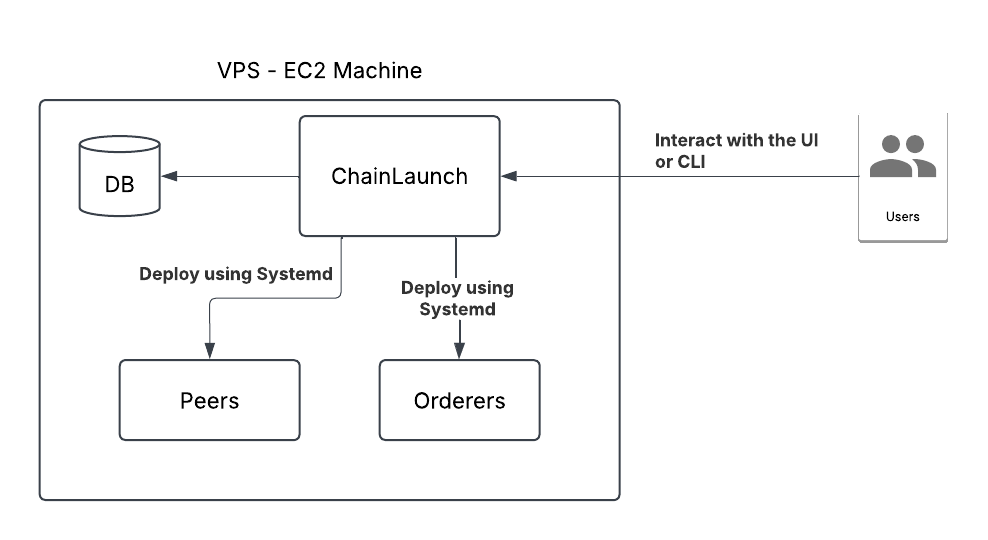
\includegraphics[width=0.95\textwidth, keepaspectratio]{Figures/Chainlaunch-architecture.png}
    \caption{Kiến trúc tổng thể của nền tảng Chainlaunch}
    \label{fig:chainlaunch-arch}
\end{figure}

\subsubsection{Công nghệ tầng Backend}

Tầng Backend đảm nhiệm toàn bộ logic nghiệp vụ, điều phối giao dịch tới mạng blockchain và quản lý dữ liệu ngoài chuỗi. Các công nghệ chủ đạo của tầng này được lựa chọn nhằm cân bằng giữa tính cấu trúc hóa của mã nguồn, độ an toàn kiểu dữ liệu và hiệu năng xử lý.

\begin{itemize}
    \item \textbf{NestJS -- Khung kiến trúc và mô hình quản trị logic:} NestJS chuẩn hóa kiến trúc máy chủ Node.js bằng cách áp dụng nghiêm ngặt mô hình \textit{Dependency Injection} (DI) và \textit{Inversion of Control} (IoC) thông qua cơ chế \textit{Decorators} và \textit{Metadata}. Nhờ đó, logic nghiệp vụ (Services) được phân tách rạch ròi khỏi logic điều phối (Controllers), giúp hệ thống đạt được tính bảo trì và khả năng kiểm thử cao. Việc tích hợp gói \pkg{@nestjs/microservices} còn cho phép trừu tượng hóa các tầng giao thức (TCP, gRPC, Redis Pub/Sub), tạo điều kiện chuyển đổi minh bạch từ mô hình đơn khối (Monolithic) sang phân tán (Microservices).

    \item \textbf{MongoDB và Prisma -- Tầng lưu trữ lai định kiểu:} MongoDB là cơ sở dữ liệu hướng tài liệu (document-oriented) phù hợp với các tập dữ liệu có cấu trúc biến đổi và yêu cầu mở rộng ngang (horizontal scaling); việc sử dụng định dạng \pkg{bson} giúp lưu trữ hiệu quả các cấu trúc phức tạp như cây Merkle. Prisma bổ khuyết nhược điểm thiếu cấu trúc của NoSQL bằng một bản đồ lược đồ (Schema) định nghĩa trước; engine của Prisma được viết bằng ngôn ngữ Rust, cung cấp khả năng tối ưu hóa truy vấn và ngăn chặn các lỗi runtime liên quan đến kiểu dữ liệu -- một yếu tố then chốt khi xử lý dữ liệu nhạy cảm như phiếu bầu.

    \item \textbf{Redis và cơ chế Cache -- Tối ưu hóa hiệu năng:} Hệ thống áp dụng mô hình lưu trữ đa tầng dựa trên công nghệ \pkg{cache-manager} và \pkg{@nestjs/cache-manager}, cho phép đồng bộ hóa trạng thái giữa các instance trong môi trường Microservices, giảm độ trễ mạng và tải trọng lên cơ sở dữ liệu chính. Redis đồng thời đóng vai trò bộ nhớ đệm trung tâm cho tác vụ giới hạn lưu lượng (Rate Limiting) thông qua \pkg{@nestjs/throttler}, giúp bảo vệ tài nguyên hệ thống trước các kịch bản tấn công khai thác hoặc quá tải truy cập nhờ tốc độ xử lý trên bộ nhớ RAM ở ngưỡng ms.
\end{itemize}

\subsubsection{Công nghệ tầng Website Frontend}

Tầng giao diện trình duyệt cung cấp môi trường tương tác cho quản trị viên và cử tri trên trình duyệt. Các công nghệ được lựa chọn nhằm tối ưu đồng thời trải nghiệm phát triển, hiệu năng tải trang và tính nhất quán về thiết kế.

\begin{itemize}
    \item \textbf{React -- Thư viện cốt lõi của tầng giao diện:} React là thư viện JavaScript được sử dụng để xây dựng giao diện người dùng theo mô hình lập trình khai báo (Declarative Programming) và kiến trúc thành phần tái sử dụng. Thông qua cơ chế đối chiếu (Reconciliation) trên DOM ảo (Virtual DOM), React xác định các thay đổi cần thiết và cập nhật chúng lên DOM thật một cách hiệu quả, từ đó giảm số lượng thao tác trực tiếp trên DOM và cải thiện hiệu năng hiển thị. Bên cạnh đó, mô hình luồng dữ liệu một chiều (Unidirectional Data Flow) cùng cơ chế truyền dữ liệu thông qua \pkg{props} giúp tăng tính minh bạch, khả năng dự đoán và khả năng bảo trì của ứng dụng.


    \item \textbf{Vite -- Công cụ xây dựng và tối ưu hóa chu kỳ phát triển:} Trong giai đoạn phát triển, Vite tận dụng tính năng ES Modules nguyên bản của trình duyệt cùng bộ biên dịch \textit{esbuild} (viết bằng ngôn ngữ Go) để loại bỏ giai đoạn đóng gói toàn bộ mã nguồn, nhờ đó giảm thời gian khởi động môi trường (Cold Start) xuống mức mili-giây. Trong giai đoạn biên dịch sản phẩm, Vite sử dụng \textit{Rollup} để thực thi các kỹ thuật phân tách mã động (Code-Splitting), loại bỏ mã thừa (Tree-Shaking) và tối ưu chiến lược tải trước tài nguyên, qua đó giữ kích thước tệp đầu ra ở mức tối thiểu và cải thiện trực tiếp các chỉ số Core Web Vitals.

    \item \textbf{Material UI và Emotion -- Hệ thống thiết kế và giải pháp CSS-in-JS:} Material UI (MUI) là thư viện giao diện người dùng cung cấp tập hợp các thành phần được xây dựng dựa trên ngôn ngữ thiết kế Material Design của Google. Kết hợp với giải pháp CSS-in-JS của Emotion (\pkg{@emotion/react} và \pkg{@emotion/styled}), MUI cho phép định nghĩa và quản lý phong cách trực tiếp trong thành phần giao diện, hạn chế xung đột giữa các lớp CSS và hỗ trợ tùy biến giao diện động trong quá trình thực thi. Bên cạnh đó, cơ chế quản lý giao diện tập trung giúp duy trì tính nhất quán về màu sắc, kiểu chữ và khoảng cách hiển thị trên toàn bộ hệ thống.

\end{itemize}

\subsubsection{Công nghệ tầng Mobile Frontend}

Tầng ứng dụng di động cho phép cử tri thực hiện bỏ phiếu trực tiếp trên thiết bị cá nhân. Để bảo đảm khả năng phát triển đa nền tảng từ một kho mã nguồn duy nhất cùng giao diện linh hoạt, tầng này được xây dựng dựa trên hai trụ cột công nghệ chính.

\begin{itemize}
    \item \textbf{Expo -- Nền tảng thực thi và quản lý vòng đời ứng dụng đa nền tảng:} Expo cung cấp giải pháp toàn diện để phát triển, biên dịch và vận hành ứng dụng trên iOS, Android và Web từ một kho mã nguồn duy nhất. Nền tảng này cung cấp các API đồng bộ giúp mã JavaScript tương tác trực tiếp với tính năng native của thiết bị (lưu trữ an toàn, định vị, camera) mà không cần can thiệp vào mã nguồn Java/Kotlin hay Objective-C/Swift. Cơ chế \textit{Expo Router} áp dụng mô hình định tuyến dựa trên tệp tin (File-based Routing), tự động hóa luồng điều hướng và tối ưu việc phân tách tài nguyên cũng như quản lý vòng đời của các màn hình.

    \item \textbf{React Native Reusables và Tailwind CSS -- Thư viện xây dựng UI:} Sự kết hợp này lấy cảm hứng trực tiếp từ mô hình \textit{Shadcn UI} trên nền tảng web, phân tách rạch ròi giữa logic vận hành và lớp trình bày của ứng dụng. Thay vì cung cấp các cấu phần đóng gói cứng nhắc, React Native Reusables (RNR) đưa cho nhà phát triển những component đơn giản (dựa trên \pkg{@rn-primitives}) đã được lập trình sẵn toàn bộ logic phức tạp bên dưới; nhà phát triển chỉ cần sao chép và tùy biến mã nguồn trực tiếp trong dự án, qua đó nắm quyền kiểm soát tuyệt đối và tránh phụ thuộc vào mã nguồn ẩn của bên thứ ba. Để hoàn thiện lớp vỏ ngoài, hệ thống sử dụng Tailwind CSS làm ngôn ngữ định kiểu theo hướng tiện ích (Utility-First): nhà phát triển chỉ cần gắn các \pkg{className} ngắn gọn để chỉ định màu sắc, khoảng cách và bố cục.
\end{itemize}

\input{Chapter-3/3.2-Tong-quan-mo-hinh-tin-cay}
\input{Chapter-3/3.3-EC-Schnorr-Blind-Multisignature}
\input{Chapter-3/3.4-JWT-hai-tang}
\input{Chapter-3/3.5-Quan-ly-session-Redis}
\input{Chapter-3/3.6-Hyperledger-Fabric}
\input{Chapter-3/3.7-Chainlaunch-Batch}
\input{Chapter-3/3.8-Merkle-Tree}
\subsection{Bảo mật tầng HTTP -- Helmet, CORS, Rate Limit và HTTPS}

Tầng HTTP là điểm tiếp xúc đầu tiên giữa cử tri và hệ thống, do đó các biện pháp phòng thủ tại tầng này được áp dụng đồng thời theo nhiều khía cạnh: \textit{tăng cường bảo mật tiêu đề HTTP} qua Helmet, giới hạn nguồn gốc qua CORS, giới hạn tần suất yêu cầu qua Rate Limiting, ngắt các yêu cầu vượt quá thời gian xử lý qua Timeout, và mã hóa truyền tải qua HTTPS.

\textbf{Helmet:} BFF và Reveal-Vote đều dùng thư viện \pkg{helmet} với cấu hình phân biệt theo môi trường (Hình~\ref{fig:helmet-config}). \textit{Content-Security-Policy} ở chế độ nghiêm ngặt với \pkg{default-src 'none'}, chỉ cho phép \pkg{connect-src 'self'} và buộc nâng cấp HTTP sang HTTPS. Các tiêu đề khác như \pkg{X-Frame-Options}, \pkg{X-Content-Type-Options}, \pkg{Referrer-Policy}, \pkg{Strict-Transport-Security}, \pkg{Cross-Origin-Opener-Policy} đều được bật mặc định.

\begin{figure}[H]
    \centering
    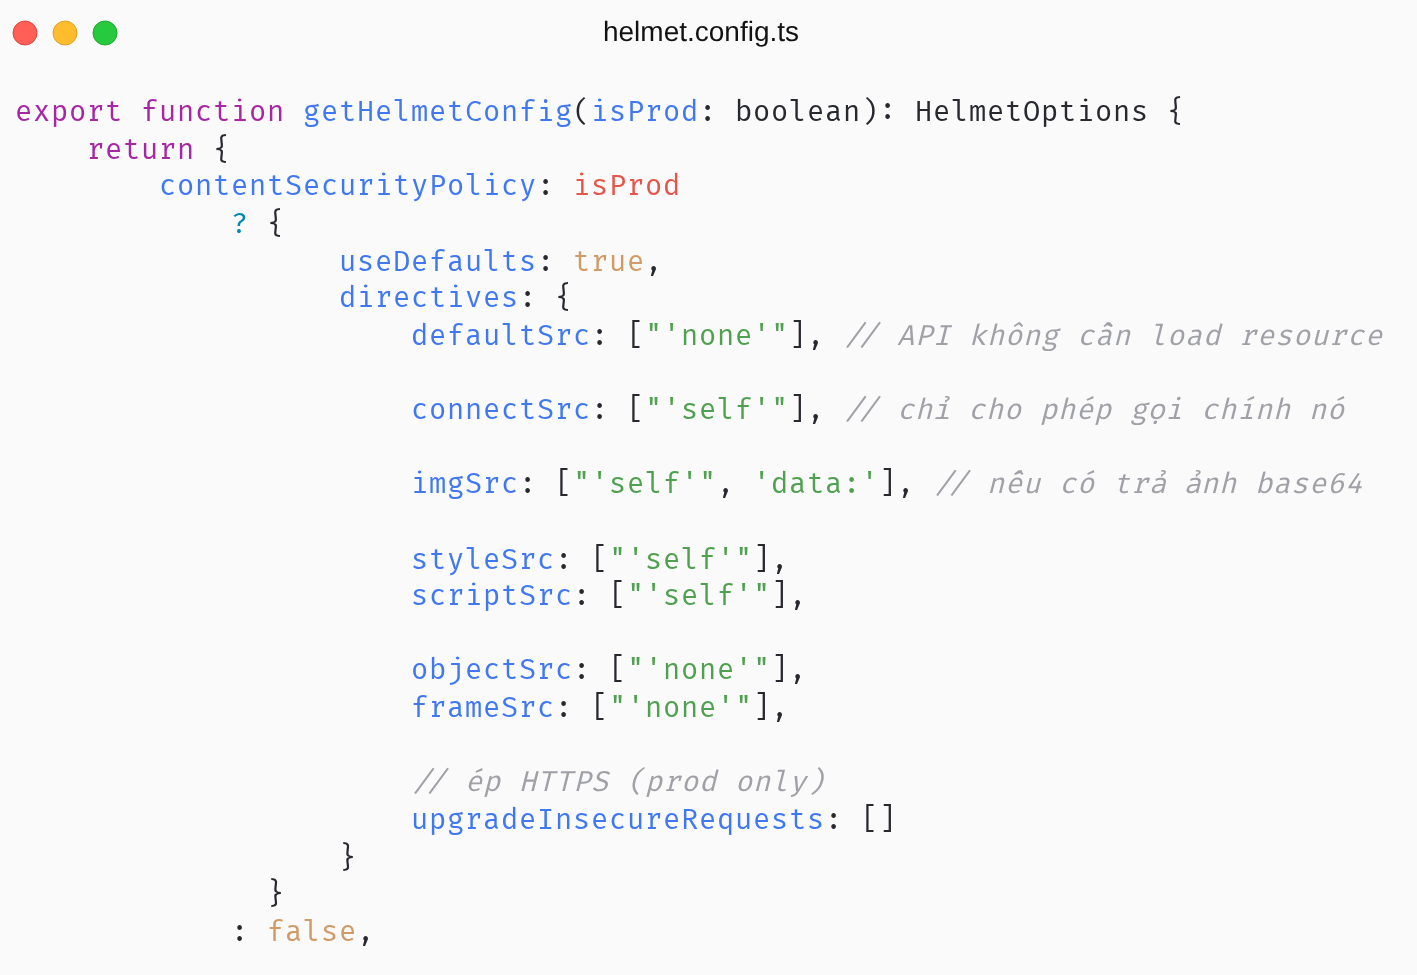
\includegraphics[width=0.85\textwidth, keepaspectratio]{Figures/code/helmet-config.png}
    \caption{Cấu hình Helmet cho môi trường sản xuất}
    \label{fig:helmet-config}
\end{figure}

\textbf{CORS:} Tiêu đề \pkg{Access-Control-Allow-Origin} chỉ chấp nhận các tên miền nằm trong biến môi trường \pkg{CORS\_ORIGINS}. Phương thức được phép giới hạn ở \pkg{GET}, \pkg{POST}, \pkg{PUT}, \pkg{PATCH}, \pkg{DELETE}, \pkg{OPTIONS}, kèm \pkg{credentials} để cookie phiên hợp lệ cho các tên miền tin cậy. Cấu hình này ngăn các trang web bên ngoài gọi API qua \pkg{XMLHttpRequest} hay \pkg{fetch} và đảm nhận một phần vai trò chống CSRF.

\textbf{Rate Limiting:} \pkg{HttpThrottlerGuard} giới hạn 100 yêu cầu mỗi IP trong mỗi 60 giây.

\textbf{Request Timeout:} \pkg{TimeoutInterceptor} áp dụng toán tử \pkg{timeout(5000)} của RxJS cho mọi yêu cầu -- sau 5 giây hệ thống trả về \pkg{408 Request Timeout} thay vì giữ kết nối vô thời hạn. Cơ chế này quan trọng khi peer Fabric phản hồi chậm: yêu cầu của cử tri không bị treo, cho phép họ thử lại thay vì chờ đợi không xác định.

\textbf{HTTPS cho BFF và Reveal-Vote:} Hai dịch vụ đều được phục vụ qua HTTPS. Hệ thống áp dụng mô hình \textit{TLS termination at edge}: một reverse proxy Cloudflare đứng trước, đảm nhận giải mã TLS rồi chuyển tiếp yêu cầu HTTP đến backend trong mạng nội bộ tin cậy. Cách triển khai này tận dụng phần cứng tăng tốc TLS của reverse proxy và giúp việc luân chuyển chứng chỉ trở nên đơn giản -- chỉ phải cập nhật tại một điểm. Trường hợp triển khai trên một máy chủ duy nhất, NestJS hỗ trợ bật HTTPS trực tiếp như sau:

\begin{figure}[H]
    \centering
    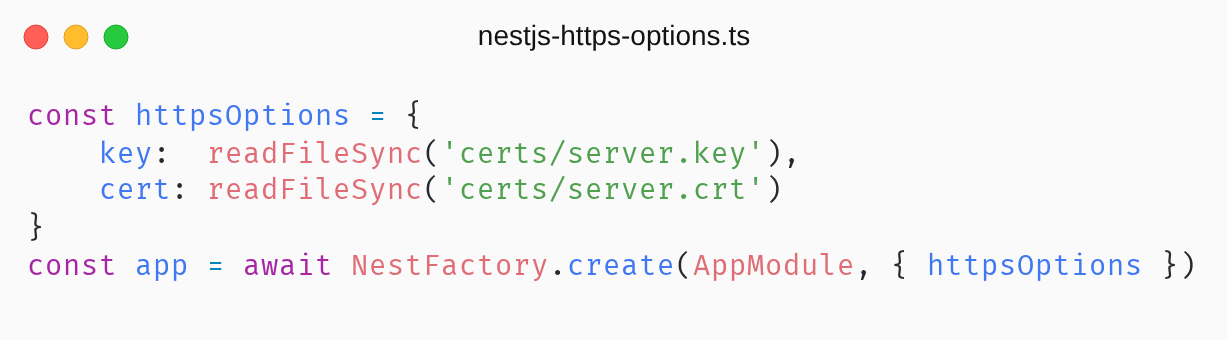
\includegraphics[width=0.70\textwidth, keepaspectratio]{Figures/code/nestjs-https-options.png}
    \caption{Khởi tạo NestJS với httpsOptions để bật HTTPS trực tiếp}
    \label{fig:nestjs-https-options}
\end{figure}

\subsection{Giao tiếp nội bộ -- TCP NestJS, mTLS và xác thực dữ liệu đầu vào}

Các dịch vụ nội bộ của hệ thống giao tiếp với nhau qua \textbf{NestJS TCP transport} thay vì REST HTTP. Cách làm này loại bỏ tầng parser HTTP, giảm độ trễ trung bình từ 5--15 ms xuống còn 1--3 ms cho mỗi vòng gọi, và quan trọng hơn -- các dịch vụ ngoài BFF và Reveal-Vote không cần mở cổng HTTP, do đó không trực tiếp tiếp xúc với mạng bên ngoài. Sơ đồ giao tiếp tổng thể được minh họa trong Hình~\ref{fig:internal-services}.

\textbf{mTLS cho kênh TCP giữa các microservice:} Do các microservice có thể được triển khai trên các máy chủ khác nhau và giao tiếp thông qua hạ tầng mạng không hoàn toàn tin cậy, hệ thống sử dụng \textit{mutual TLS} (mTLS) để mã hóa dữ liệu truyền tải và xác thực hai chiều danh tính dịch vụ. Nhờ đó, chỉ những dịch vụ sở hữu chứng chỉ hợp lệ mới có thể tham gia trao đổi dữ liệu. Cấu hình microservice của NestJS được khởi tạo với \pkg{tlsOptions}:

\begin{figure}[H]
    \centering
    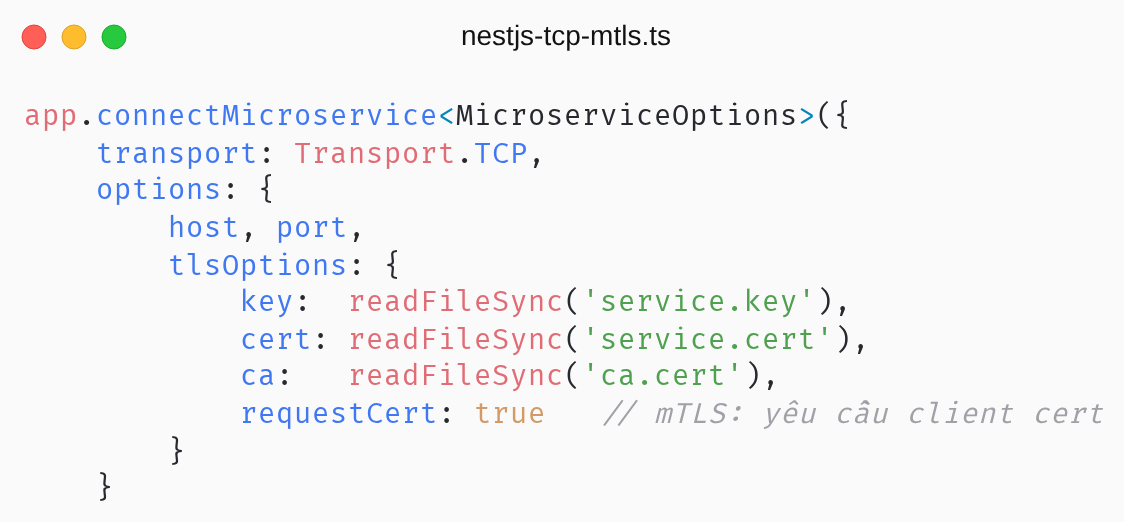
\includegraphics[width=0.75\textwidth, keepaspectratio]{Figures/code/nestjs-tcp-mtls.png}
    \caption{Cấu hình mTLS cho NestJS TCP microservice với tlsOptions}
    \label{fig:nestjs-tcp-mtls}
\end{figure}

\textbf{Xác thực dữ liệu đầu vào:} Mọi yêu cầu vào hệ thống -- cả từ trình duyệt qua HTTP đến BFF lẫn từ microservice qua kênh TCP -- đều được kiểm chứng tự động qua \pkg{ValidationPipe} toàn cục. Lớp DTO khai báo các ràng buộc dưới dạng decorator của \pkg{class-validator}: \pkg{@IsDefined}, \pkg{@IsString},... Ví dụ điển hình là \pkg{SignInDto} và \pkg{RefreshTokenDto} trong Hình~\ref{fig:class-validator-dto}.

\begin{figure}[H]
    \centering
    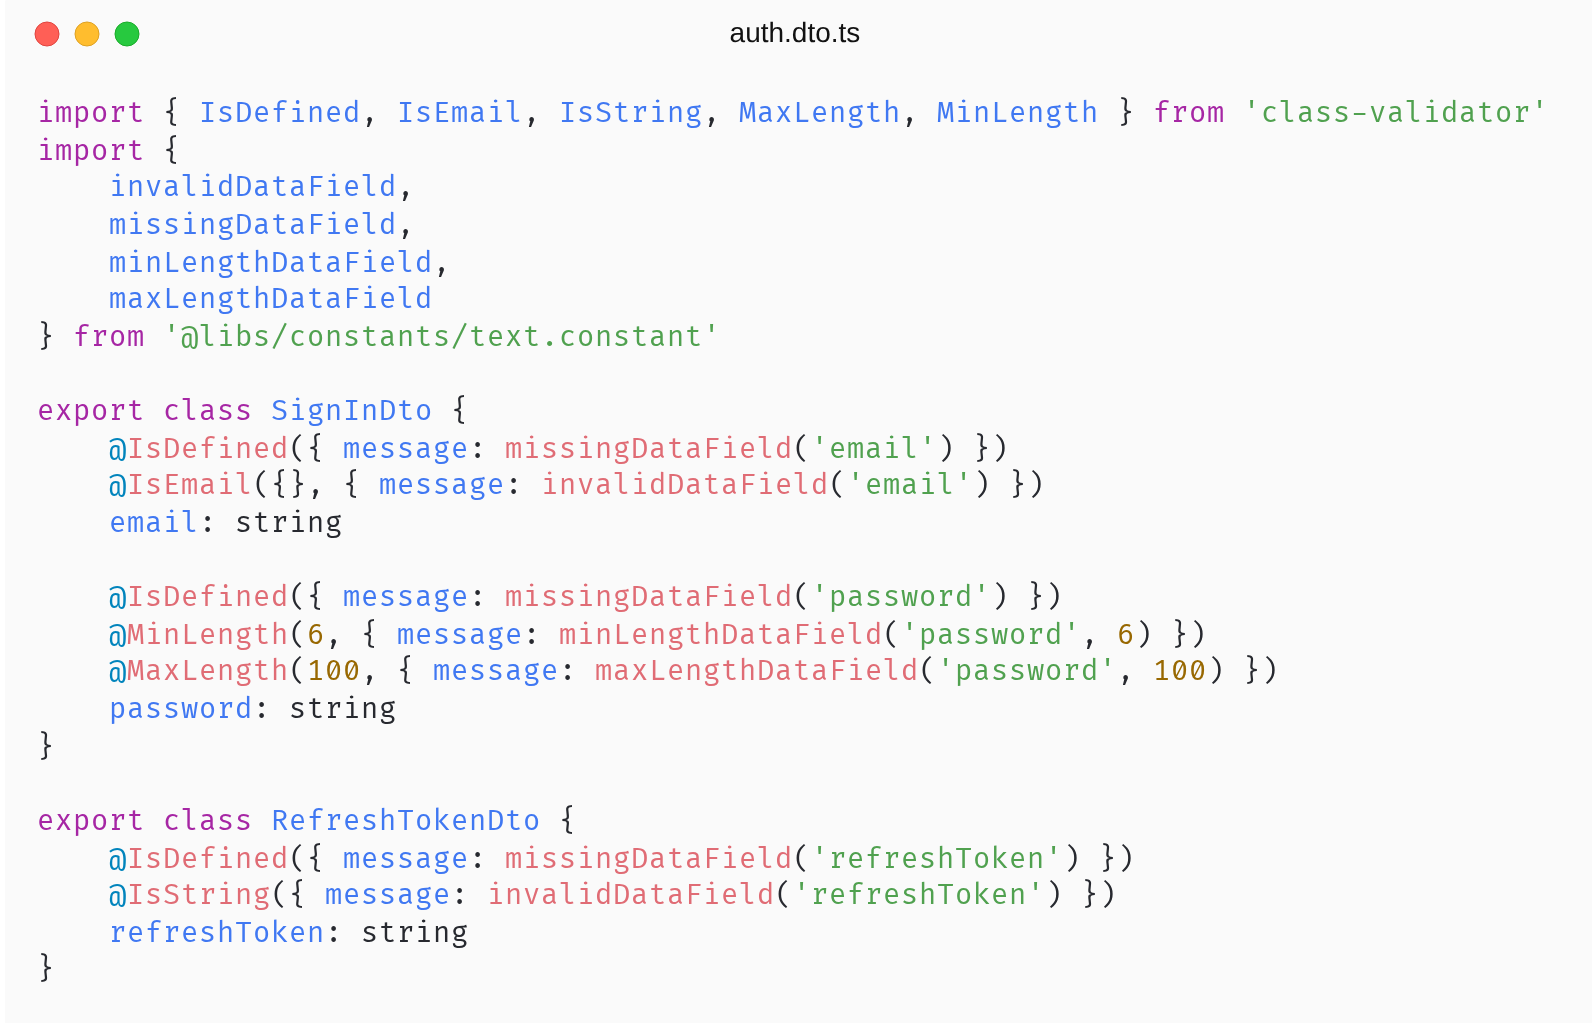
\includegraphics[width=0.85\textwidth, keepaspectratio]{Figures/code/class-validator-dto.png}
    \caption{DTO xác thực dữ liệu vào bằng decorator của class-validator}
    \label{fig:class-validator-dto}
\end{figure}

\input{Chapter-3/3.11-AES-256-GCM}
\subsection{Tối ưu hiệu năng hệ thống}

Một số kỹ thuật tối ưu hiệu năng được áp dụng nhằm giữ độ trễ ở mức chấp nhận được dưới tải bầu cử đỉnh -- khi hàng nghìn cử tri có thể đồng thời bỏ phiếu trong cùng một khoảng thời gian ngắn.

\textbf{MongoDB Replica Set và Prisma transaction:} Cụm MongoDB được khởi tạo với \pkg{--replSet rs0}, là điều kiện bắt buộc để Prisma sử dụng \pkg{\$transaction} với nhiều thao tác ACID. Hệ thống tuân thủ \textit{kiểm tra hợp lệ ngoài giao dịch, chỉ ghi (commit) trong giao dịch}: các thao tác đọc và side-effect nặng (gọi Fabric mất 2--3 giây) được thực hiện \textbf{ngoài} giao dịch; giao dịch chỉ chứa hai bước \textit{re-validate} (chống xung đột đồng thời) và \textit{ghi}. Nhờ đó thời gian giữ khóa của giao dịch ngắn, thông lượng tăng đáng kể so với cách bao bọc toàn bộ luồng nghiệp vụ.

\textbf{Cache phản hồi HTTP:} \pkg{HttpCacheInterceptor} đệm phản hồi của các yêu cầu \pkg{GET} vào Redis. Các endpoint danh sách bầu cử công khai và xem chi tiết ứng viên hưởng lợi nhiều nhất từ cơ chế này vì chúng có tải đọc cao và dữ liệu thay đổi ít.

\textbf{Chiến lược chỉ mục MongoDB:} Các bảng chính được phủ chỉ mục để mọi thao tác đọc theo dõi được $O(\log N)$ hoặc $O(1)$ thay vì quét tuần tự. Bảng~\ref{tab:mongo-index} liệt kê các chỉ mục then chốt.

\begin{table}[H]
\centering
\caption{Chiến lược chỉ mục các bảng chính trong MongoDB}
\label{tab:mongo-index}
\begin{tabularx}{\textwidth}{|L{0.2}|L{0.4}|L{0.4}|}
\hline
\textbf{Bảng} & \textbf{Chỉ mục} & \textbf{Mục đích} \\
\hline
\pkg{elections} & \pkg{(status, startDate, endDate)} & Lọc bầu cử theo trạng thái và thời gian \\
\hline
\pkg{election\_voters} & \pkg{unique(electionId, voterId)} & Tra cứu O(1) và loại bỏ phần tử trùng lặp \\
\hline
\pkg{votes} & \pkg{unique(electionId, voterId)} & Chống bỏ phiếu hai lần \\
 & \pkg{unique(electionId, blindedCommitment)} & Chống nộp commitment trùng \\
 & \pkg{(electionId, createdAt)} & Lấy theo thứ tự cho cây Merkle \\
\hline
\pkg{revealed\_votes} & \pkg{unique(electionId, revealKey)} & Chống phát lại reveal \\
 & \pkg{(electionId, candidateId)} & Tổng hợp kết quả theo ứng viên \\
\hline
\end{tabularx}
\end{table}

\textbf{Truy vấn song song:} Những tác vụ độc lập không phụ thuộc lẫn nhau được thực thi đồng thời bằng \pkg{Promise.all}. Ví dụ, khi hiển thị kết quả bầu cử, hệ thống đồng thời lấy dữ liệu từ MongoDB, Coordinator Service và Hyperledger Fabric thay vì chờ từng truy vấn hoàn thành tuần tự. Nhờ đó, thời gian phản hồi chỉ phụ thuộc vào truy vấn chậm nhất, giúp giảm đáng kể độ trễ khi tải dữ liệu.

\subsection{Nhất quán dữ liệu giữa blockchain và MongoDB}

Mỗi thao tác nghiệp vụ quan trọng của hệ thống đều phải ghi đồng thời lên hai hệ lưu trữ tách biệt: sổ cái Hyperledger Fabric và cơ sở dữ liệu MongoDB. Hai lần ghi này không thể bọc chung trong một giao dịch nguyên tử (\textit{atomic}). Nếu ghi chuỗi khối trước rồi ghi cơ sở dữ liệu sau (\textit{chain-first}), một lỗi xảy ra ở bước ghi cơ sở dữ liệu — \textbf{sau khi} chuỗi khối đã ghi nhận thành công — sẽ làm hai bên lệch nhau; và vì sổ cái là bất biến nên không thể hoàn tác. Bảng~\ref{tab:dual-write} liệt kê ba điểm ghi kép cùng hậu quả khi lệch theo hướng \textit{chain-first}.

\begin{table}[H]
\centering
\caption{Ba điểm ghi kép và hậu quả khi lệch dữ liệu theo hướng chain-first}
\label{tab:dual-write}
\begin{tabularx}{\textwidth}{|L{0.32}|L{0.68}|}
\hline
\textbf{Thao tác} & \textbf{Hậu quả khi chuỗi khối thành công nhưng cơ sở dữ liệu lỗi} \\
\hline
\pkg{SubmitVote} & Chuỗi khối có phiếu, cơ sở dữ liệu thiếu $\rightarrow$ số phiếu hai bên lệch $\rightarrow$ lệnh \pkg{CommitMerkleRoot} bị từ chối khi đóng cuộc bầu cử. \\
\hline
\pkg{CommitMerkleRoot} & Chuỗi khối đã đóng, cơ sở dữ liệu còn \pkg{ACTIVE} $\rightarrow$ thử lại bị từ chối (do tính idempotent) $\rightarrow$ cuộc bầu cử bị kẹt. \\
\hline
\pkg{RevealVoteCompact} & Chuỗi khối đã dùng \pkg{revealKey}, cơ sở dữ liệu thiếu $\rightarrow$ cử tri thử lại bị báo ``revealKey đã dùng'' $\rightarrow$ không thể tiết lộ lại. \\
\hline
\end{tabularx}
\end{table}

\subsubsection{Giải pháp 1 --- Ghi cơ sở dữ liệu trước kèm trạng thái trung gian}

Hai thao tác \pkg{SubmitVote} và đóng cuộc bầu cử áp dụng mô hình \textit{Write-DB-First}: ghi cơ sở dữ liệu ở một trạng thái trung gian \textbf{trước}, rồi mới gọi chuỗi khối, sau đó xác nhận lại cơ sở dữ liệu. Trình tự gồm bốn bước:

\begin{itemize}
    \item \textbf{Bước 1 --- Ghi trạng thái trung gian:} ghi bản ghi với trạng thái \pkg{Vote.status = PENDING\_CHAIN} (đối với phiếu) hoặc \pkg{Election.status = CLOSING} (đối với đóng cuộc bầu cử), trường \pkg{blockchainRef} để trống. Vì cơ sở dữ liệu được ghi trước, ràng buộc duy nhất \pkg{(electionId, voterId)} chặn bỏ phiếu trùng ngay tại bước này — trước cả khi chạm tới chuỗi khối; riêng \pkg{CLOSING} còn đóng vai trò khóa chống đóng cuộc bầu cử đồng thời.

    \item \textbf{Bước 2 --- Gọi chuỗi khối:} thực thi giao dịch \textit{invoke} tương ứng.

    \item \textbf{Bước 3 --- Chuỗi khối thành công:} xác nhận cơ sở dữ liệu, chuyển trạng thái sang \pkg{CONFIRMED} (hoặc \pkg{CLOSED}) và ghi \pkg{blockchainRef} bằng mã giao dịch trả về.

    \item \textbf{Bước 4 --- Chuỗi khối báo lỗi:} truy vấn lại chuỗi khối (\pkg{GetVote} hoặc \pkg{GetMerkleRoot}) để phân định, vì chuỗi khối là \textbf{nguồn sự thật}: nếu dữ liệu \textit{đã} có trên chuỗi khối thì xác nhận cơ sở dữ liệu và phục hồi mã giao dịch từ kết quả truy vấn; nếu \textit{chưa} có thì hoàn tác cơ sở dữ liệu (xóa phiếu \pkg{PENDING\_CHAIN} hoặc đưa cuộc bầu cử về \pkg{ACTIVE}) rồi ném lỗi để người dùng thử lại.
\end{itemize}

Hình~\ref{fig:submit-vote-write-db-first} trình bày hiện thực của mô hình này trong thao tác nộp phiếu.

\begin{figure}[H]
    \centering
    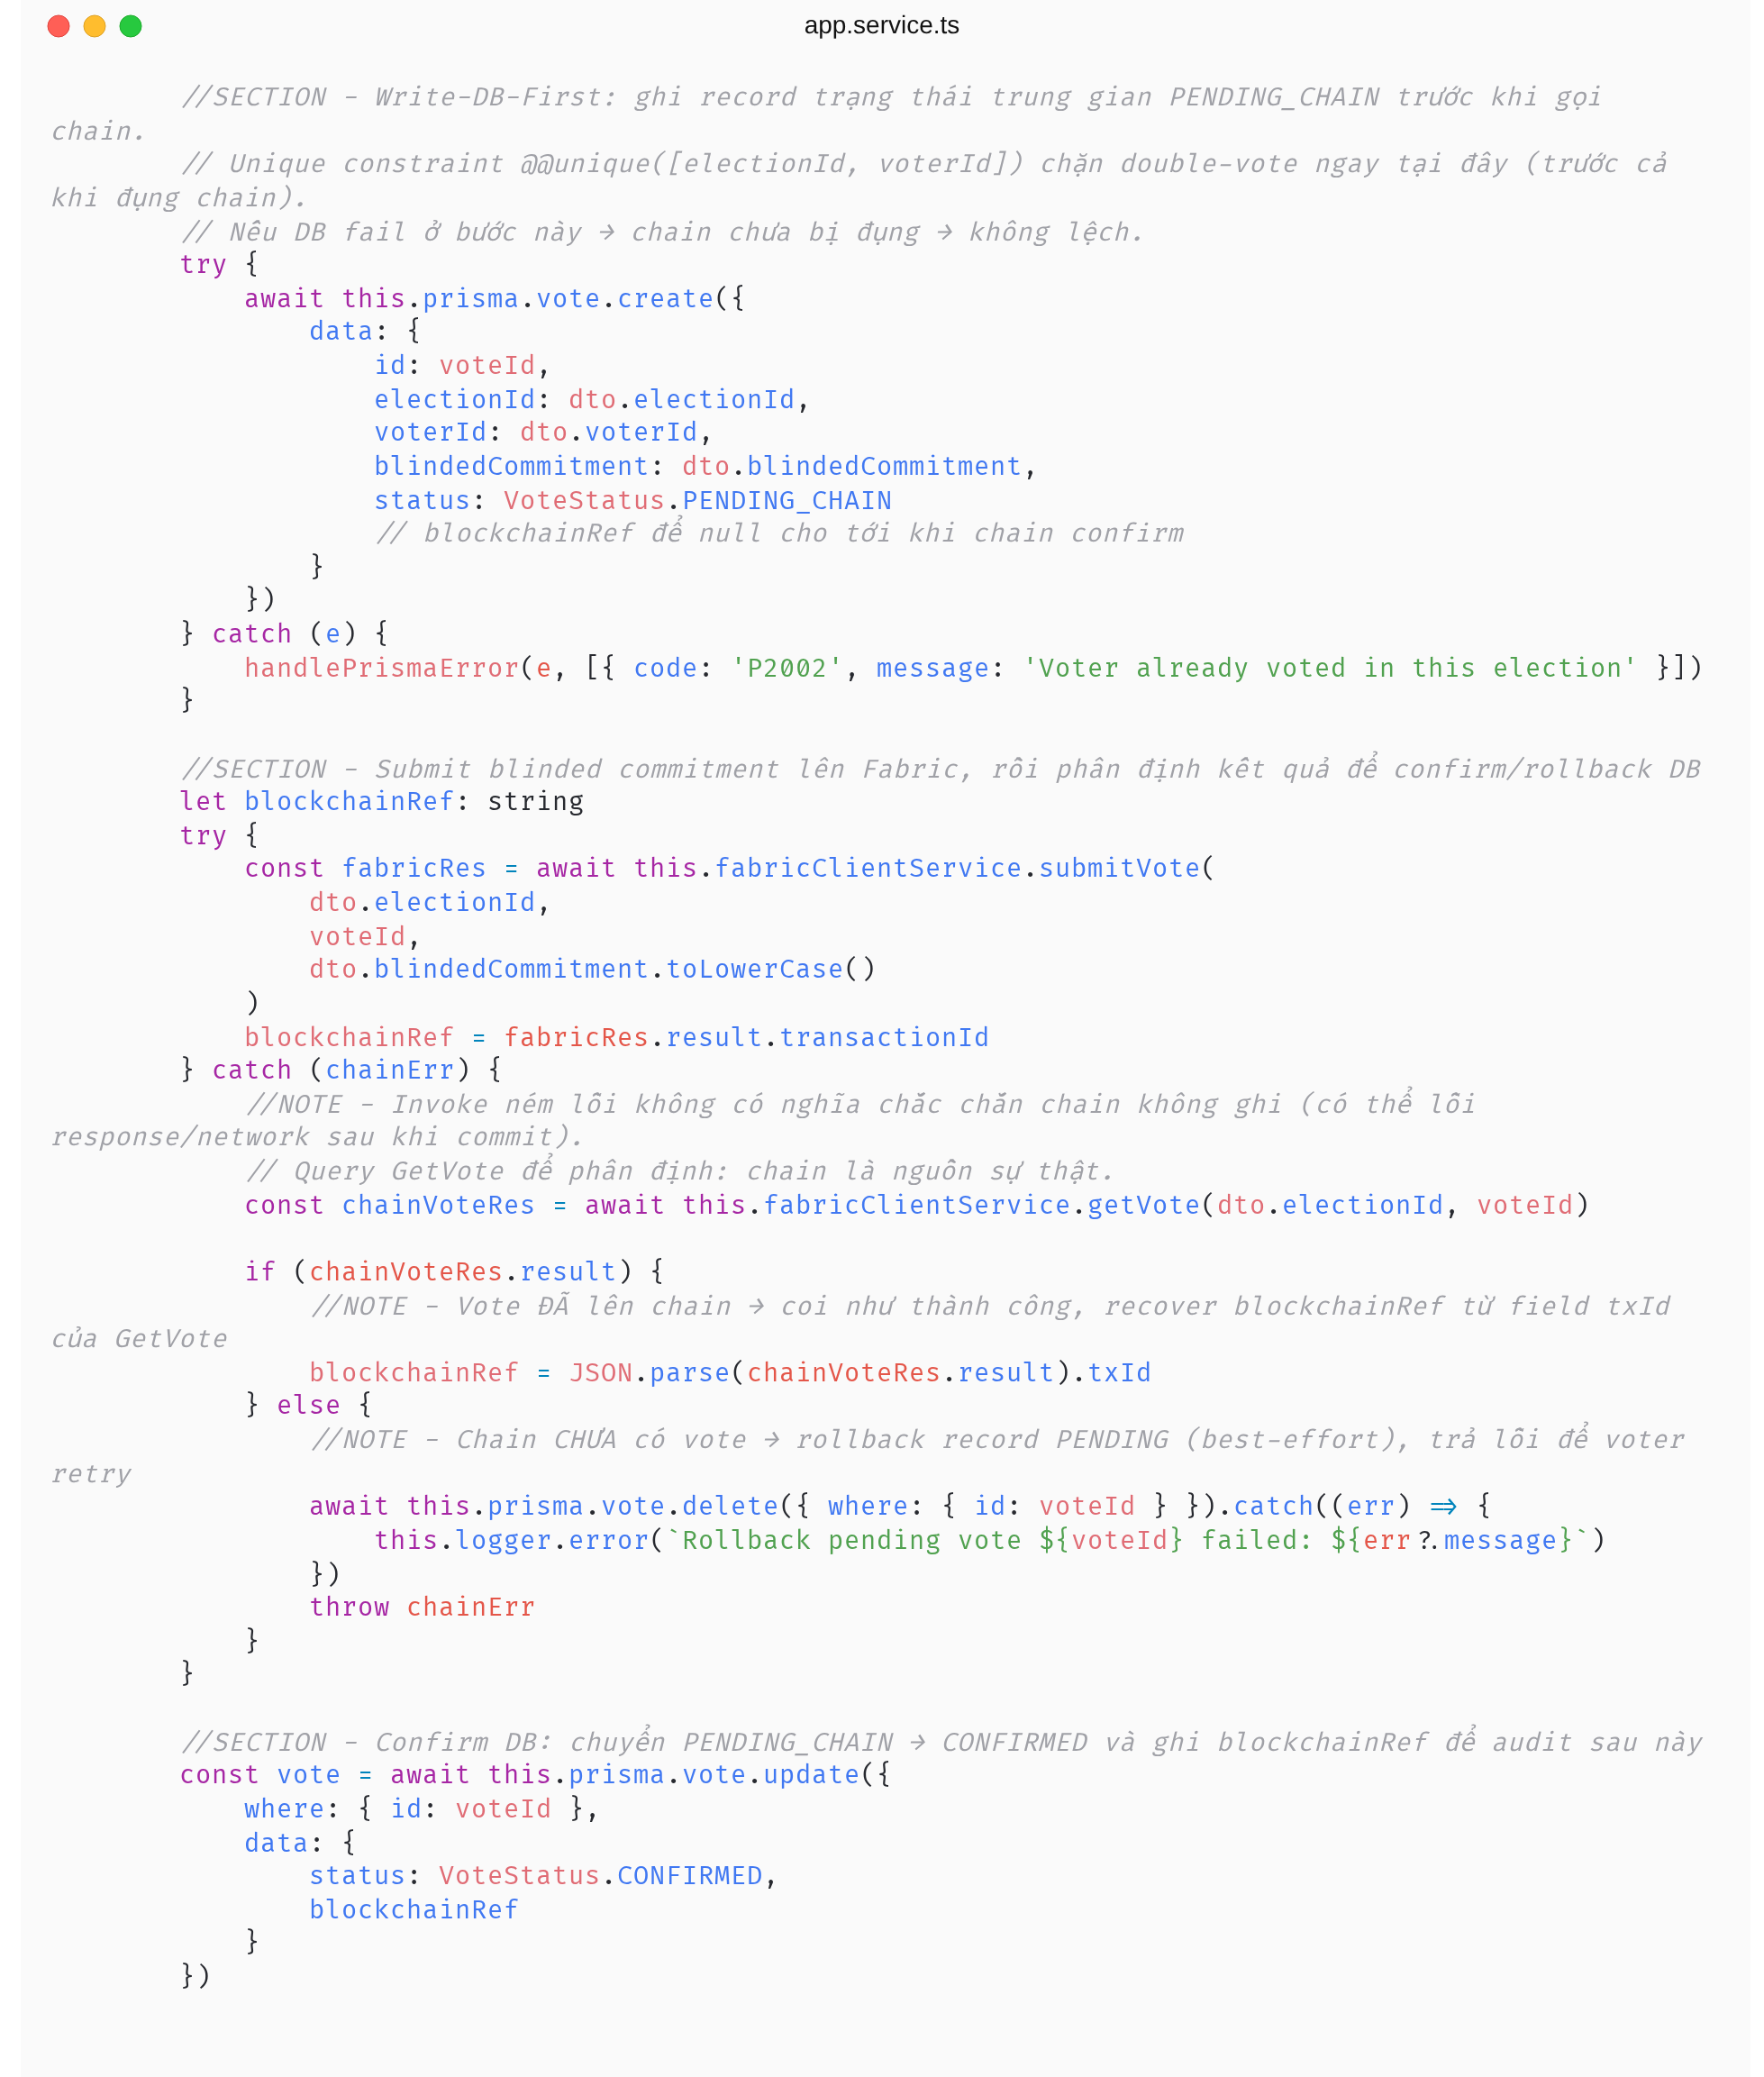
\includegraphics[width=\textwidth, keepaspectratio]{Figures/code/submit-vote-write-db-first.png}
    \caption{Mô hình Write-DB-First trong thao tác nộp phiếu \pkg{submitBlindedCommitment}}
    \label{fig:submit-vote-write-db-first}
\end{figure}

\subsubsection{Giải pháp 2 --- Giữ chain-first kèm tự phục hồi khi thử lại}

Thao tác \pkg{RevealVoteCompact} không đổi thứ tự ghi (vẫn chuỗi khối trước, cơ sở dữ liệu sau) vì \pkg{revealKey} là khóa idempotent tự nhiên trên chuỗi khối. Khi lệnh \textit{invoke} báo lỗi, hệ thống truy vấn \pkg{GetUsedReveal}: nếu chuỗi khối \textit{chưa} có \pkg{revealKey} thì đây là lỗi thật, ném tiếp; nếu chuỗi khối \textit{đã} có (và danh sách ứng viên khớp) thì coi là thử lại sau lỗi một phần, hệ thống ghi lại bản ghi cơ sở dữ liệu với \pkg{blockchainRef} để trống. Ràng buộc duy nhất \pkg{(electionId, revealKey)} vẫn ném lỗi nếu cơ sở dữ liệu đã có bản ghi, do đó tấn công phát lại thật vẫn bị chặn — chỉ phục hồi khi cơ sở dữ liệu còn trống.

\subsubsection{Tiến trình đồng bộ nền (Reconciler)}

Hai giải pháp trên xử lý lỗi trong luồng đồng bộ của yêu cầu. Trường hợp tiến trình \textit{sập} giữa bước gọi chuỗi khối và bước xác nhận sẽ để lại bản ghi kẹt ở trạng thái trung gian. Một tiến trình đồng bộ nền (\textit{reconciler}) chạy theo lịch \pkg{@Cron} của \pkg{@nestjs/schedule} đảm nhiệm việc dọn dẹp: định kỳ quét các bản ghi kẹt \textbf{cũ hơn} một ngưỡng thời gian (tránh tranh chấp với yêu cầu đang chạy), có cờ chống chồng lấn chu kỳ:

\begin{itemize}
    \item Phiếu còn \pkg{PENDING\_CHAIN}: truy vấn \pkg{GetVote} --- nếu có trên chuỗi khối thì chuyển \pkg{CONFIRMED}, nếu không thì xóa bản ghi.
    \item Cuộc bầu cử còn \pkg{CLOSING}: truy vấn \pkg{GetMerkleRoot} --- nếu đã cố định thì chuyển \pkg{CLOSED} và phục hồi mã giao dịch, nếu không thì giữ nguyên chờ quản trị viên thử lại.
\end{itemize}

\begin{figure}[H]
    \centering
    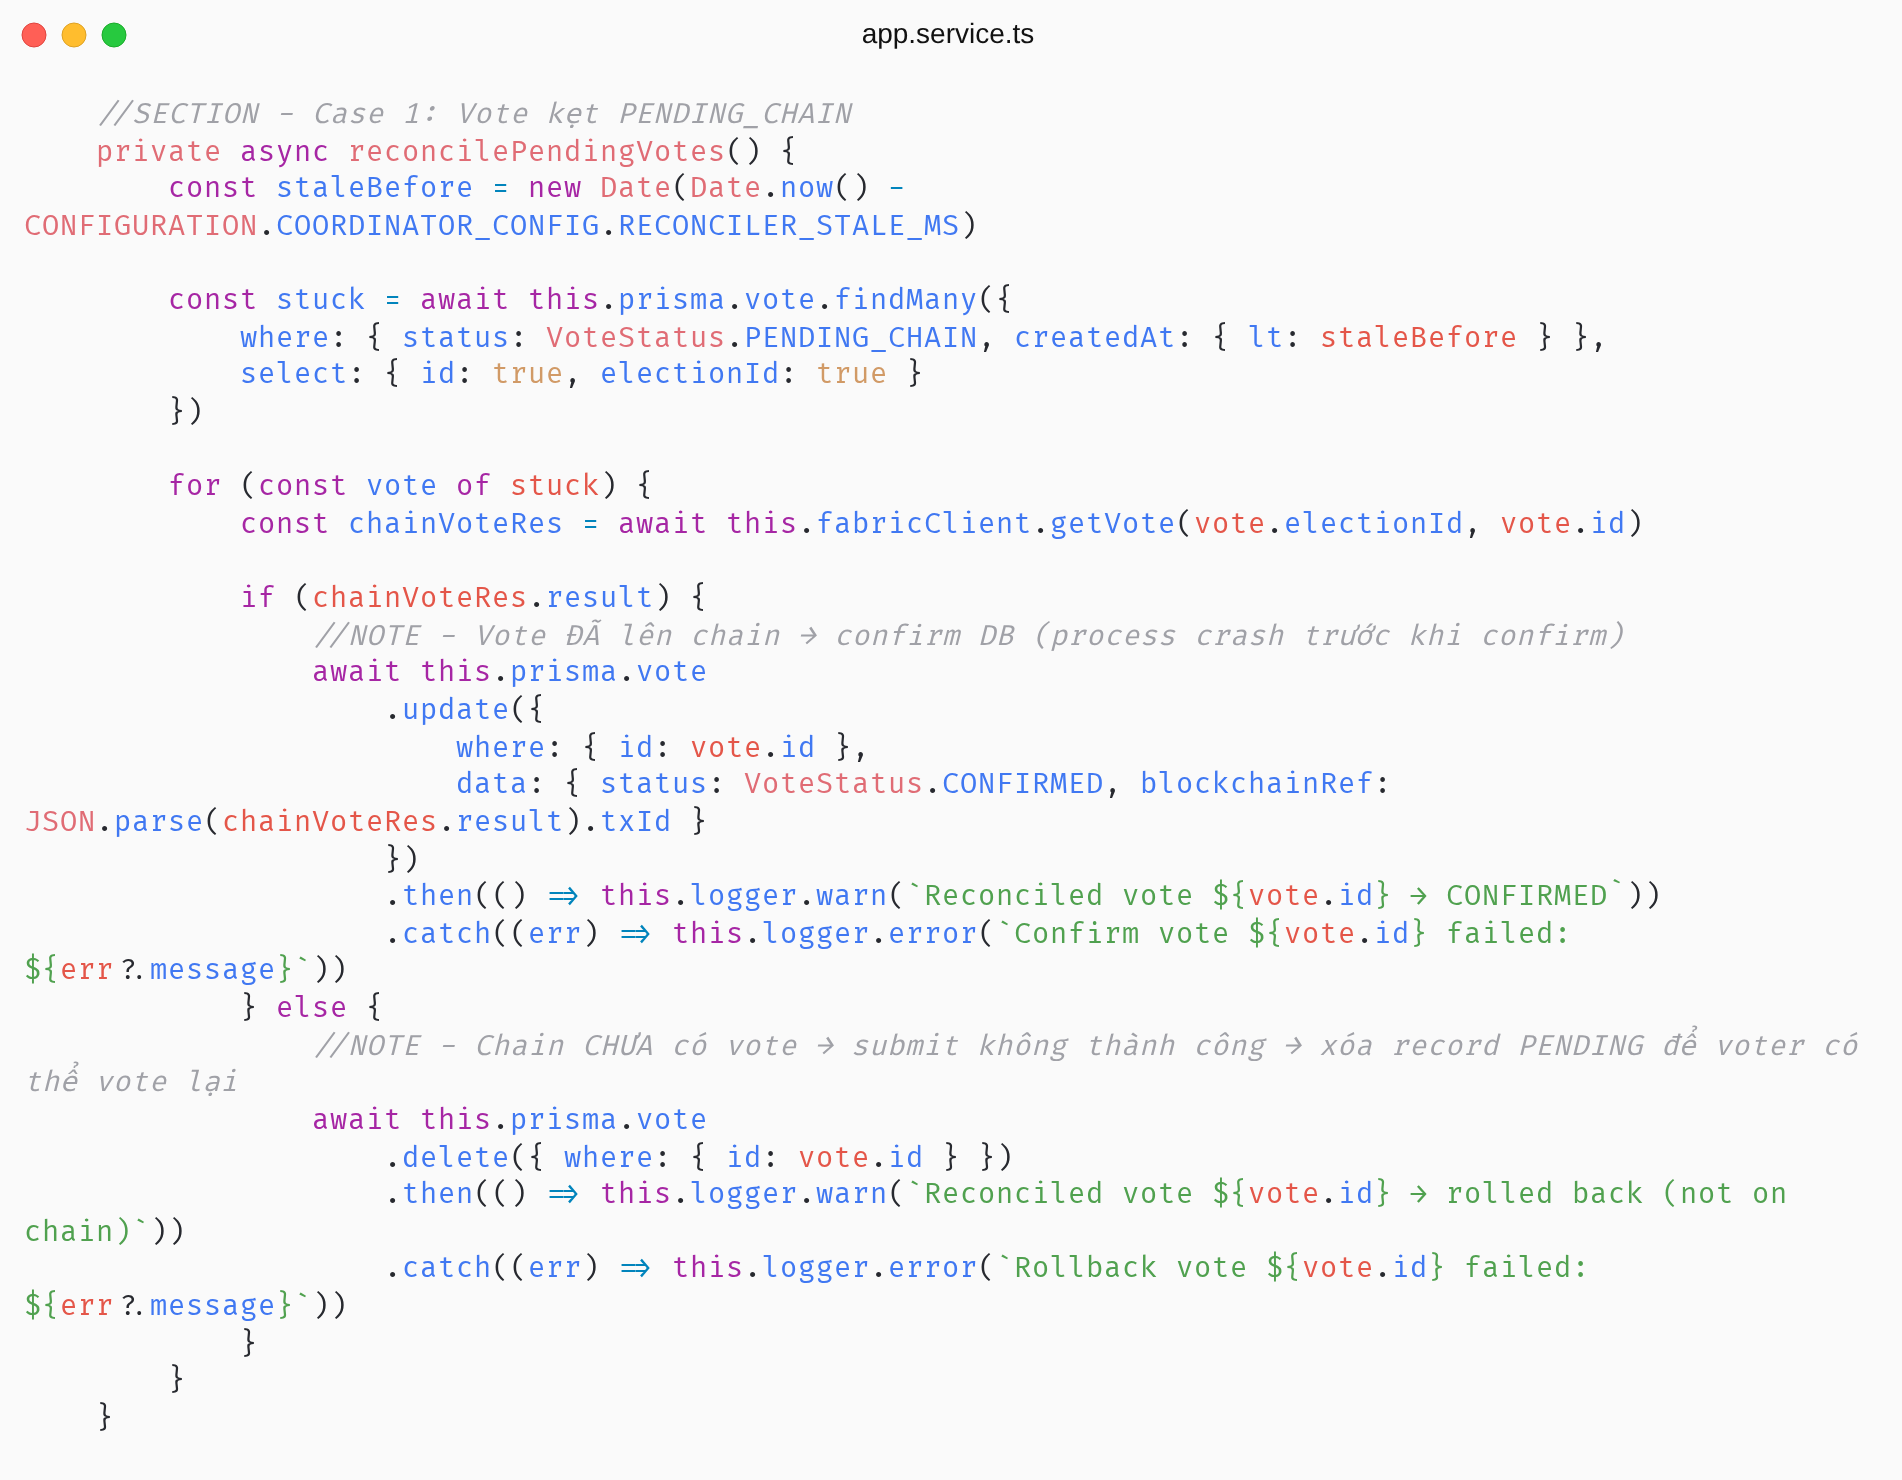
\includegraphics[width=\textwidth, keepaspectratio]{Figures/code/reconciler-pending-vote.png}
    \caption{Tiến trình đồng bộ nền đối chiếu phiếu \pkg{PENDING\_CHAIN} với chuỗi khối}
    \label{fig:reconciler-pending-vote}
\end{figure}

\subsubsection{Hệ quả về bất biến đọc dữ liệu}

Do chuỗi khối là nguồn sự thật, một phiếu chỉ được coi là hợp lệ khi đã \pkg{CONFIRMED}. Vì vậy mọi hàm đọc phiếu (đếm phiếu, dựng cây Merkle khi đóng, lọc danh sách phiếu) đều \textbf{mặc định lọc} \pkg{status = CONFIRMED} để khớp đúng tập phiếu thực sự có trên chuỗi khối. Hai ngoại lệ được giữ \textit{không phụ thuộc trạng thái} một cách có chủ đích: kiểm tra bỏ phiếu trùng khi khởi tạo phiên (phiếu \pkg{PENDING\_CHAIN} vẫn phải tính là ``đã bỏ phiếu'' để giữ chỗ) và thao tác xác minh phiếu phục vụ điều tra (cần thấy cả phiếu \pkg{PENDING\_CHAIN} để phát hiện lệch dữ liệu). Đây là mô hình \textit{nhất quán cuối} (\textit{eventual consistency}): trong khoảng chuỗi khối tạm thời không phản hồi, một phiếu có thể nằm ở \pkg{PENDING\_CHAIN} cho tới khi tiến trình đồng bộ nền đưa nó về trạng thái cuối cùng.

\subsection{Sao lưu và khôi phục khóa bí mật phiếu}

Sau khi bỏ phiếu, cử tri giữ một tập \textit{khóa bí mật phiếu} ngay trên thiết bị di động — gồm các hệ số làm mù $(\alpha, \beta)$, hai thành phần chữ ký $(h, s')$ và danh sách ứng viên đã chọn — được lưu trong kho lưu trữ an toàn (\textit{Secure Store}) của hệ điều hành. Tập khóa này là điều kiện bắt buộc để cử tri tiết lộ phiếu và tự xác minh phiếu về sau; mất thiết bị đồng nghĩa mất vĩnh viễn khả năng đó. Hệ thống vì vậy cung cấp cơ chế sao lưu và khôi phục các khóa này lên máy chủ mà vẫn không làm suy giảm tính bí mật, theo mô hình \textit{zero-knowledge}.

\subsubsection{Lớp mã hóa phía máy khách (zero-knowledge)}

Toàn bộ việc mã hóa diễn ra trên thiết bị, trước khi bất kỳ dữ liệu nào rời khỏi máy khách. Cử tri đặt một mã PIN; ứng dụng dẫn xuất khóa đối xứng 256-bit từ mã PIN bằng hàm \pkg{PBKDF2-SHA256} với $100{,}000$ vòng lặp và một salt ngẫu nhiên, sau đó mã hóa tập khóa bằng \pkg{AES-256-GCM}. Kết quả là một gói dữ liệu (\textit{envelope}) JSON chứa tham số dẫn xuất khóa (thuật toán, số vòng, salt) và phần bản mã (vector khởi tạo, bản mã kèm thẻ xác thực). Vì máy chủ \textbf{không bao giờ nhận mã PIN}, máy chủ không thể dẫn lại khóa nên không thể giải lớp mã hóa này. Số vòng lặp lớn của PBKDF2 làm chậm đáng kể tấn công dò mã PIN theo kiểu vét cạn. Hình~\ref{fig:backup-derive-key} trình bày hàm dẫn xuất khóa và mã hóa gói envelope.

\begin{figure}[H]
    \centering
    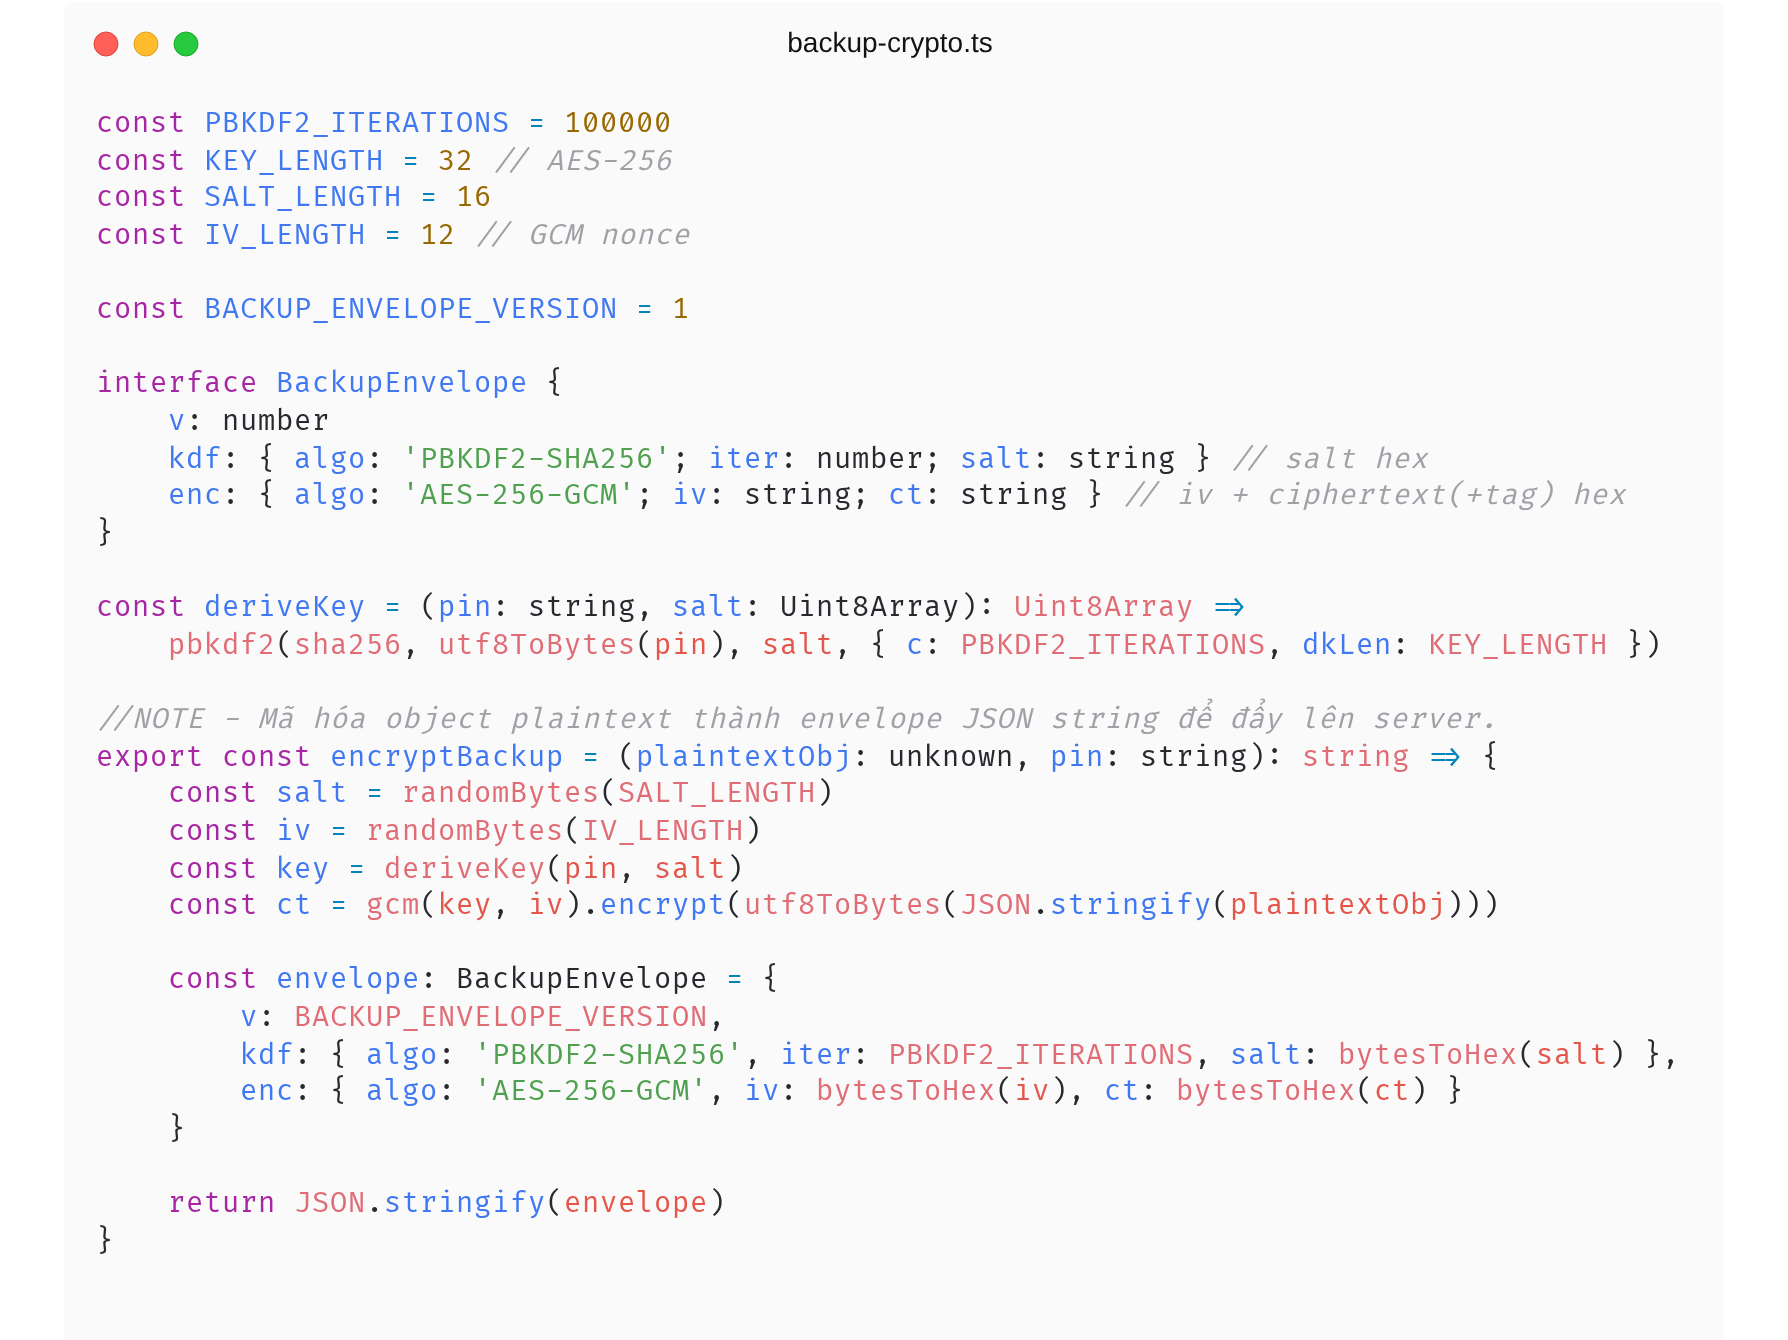
\includegraphics[width=\textwidth, keepaspectratio]{Figures/code/backup-derive-key.png}
    \caption{Hàm dẫn xuất khóa từ mã PIN bằng PBKDF2-SHA256 và mã hóa gói sao lưu bằng AES-256-GCM phía máy khách}
    \label{fig:backup-derive-key}
\end{figure}

\subsubsection{Lớp mã hóa dữ liệu khi lưu trữ (\textit{at-rest encryption}) phía máy chủ}

Khi nhận được gói envelope, Identity Service áp dụng thêm \textbf{một lớp mã hóa thứ hai} trước khi ghi xuống MongoDB nhằm bảo vệ dữ liệu khi lưu trữ. Lớp này dẫn xuất khóa bằng \pkg{argon2id} từ một bí mật phía máy chủ \pkg{BACKUP\_SECRET} kết hợp một salt ngẫu nhiên theo từng bản ghi, rồi mã hóa bằng \pkg{AES-256-GCM}. Như vậy, một bản sao lưu chịu hai lớp mã hóa độc lập: lớp ngoài chỉ giải được bằng mã PIN của cử tri, lớp trong chỉ giải được khi máy chủ nắm \pkg{BACKUP\_SECRET}. Kẻ tấn công đọc trộm cơ sở dữ liệu sẽ không thu được gì nếu thiếu cả hai bí mật này.

\subsubsection{Khôi phục và lưu ý vận hành}

Khi khôi phục, Identity Service gỡ lớp mã hóa dữ liệu khi lưu trữ và trả lại gói envelope nguyên bản do máy khách tạo; ứng dụng dẫn lại khóa từ mã PIN và giải mã. Nhờ \pkg{AES-256-GCM} là mã hóa có xác thực (\textit{authenticated encryption}), một mã PIN sai sẽ khiến bước kiểm tra thẻ xác thực thất bại ngay tại máy khách và ứng dụng báo lỗi ``Mã PIN không đúng'' — máy chủ không tham gia và cũng không học được bất kỳ thông tin nào về mã PIN.

Về vận hành, biến môi trường \pkg{BACKUP\_SECRET} của Identity Service phải được đặt bằng một giá trị mạnh trong môi trường sản xuất; giá trị mặc định dự phòng chỉ phục vụ phát triển cục bộ. Lý tưởng nhất, bí mật này nên được quản lý bởi một kho bí mật chuyên dụng thay vì lưu trong tệp cấu hình.

\input{Chapter-3/3.15-Ket-luan-chuong}
